%\documentclass[multi,preview,varwidth=false,border=5,12pt]{standalone}
\documentclass[12pt]{article}

\newcounter{Qnum}
\usepackage{assignments}
%\standaloneenv{question}


\excludecomment{solution}\let\endsolution\relax


\begin{document}

\begin{center}
\section*{Forces, drag and lift}
\end{center}

\begin{question}

Consider steady, incompressible flow through the device shown.  Determine the magnitude and direction of the weight flow rate through port 3 if sea water enters port 1 with a volume flow rate of 2 $\ft^3/s$ and exits port 2 with a velocity of 72 $\ft/s$.  Take the areas of the ports to be $A_1=2~\inch^2$, $A_2=1~\inch^2$, and $A_3=0.75~\inch^2$.

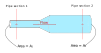
\includegraphics[width=3in]{imgs/continuity.pdf}

\begin{solution}
\begin{align*}
W_3 &=\gamma Q_1-\gamma A_2 v_2=\gamma\left(Q_1-A_2 v_2\right) \\
&=\gamma\left(2~\ft^3/s-0.5~\ft^3/s\right)=\gamma \left(1.5~\ft^3/s\right)\\
&=(64.27~\lb/\ft^3)(1.5~\ft^3/s)=96.4~\lb/s
\end{align*}
\end{solution}

\end{question}


\begin{question}

What force is required to hold a flat plate in equilibrium perpendicular to the flow of a $1~\cm$ diameter jet of water having a velocity of $3~\m/s$?  Report your result in Newtons.

\end{question}

\begin{question}

In this problem we will estimate the force from an 80~mph wind gust on a highway sign that is $12~\ft$ wide by $3~\ft$ high.  Assume the wind is flowing perpendicular to the face of the sign.  Take the air temperature to be $-20\F$ where $\rho=2.68\times 10^{-3}~\slug/\ft^3$.

First compute the force on the sign using the Force Equation $F=\rho Q \Delta v$.  Assume the air leaves parallel to the face of the sign.

Next compute the drag force using a drag coefficient $C_D=1.16$.

These should agree within a factor of two.  Do you trust one calculation more than the other?

\end{question}

\begin{question}

Compute the force required to hold a $90^\circ$ standard elbow in place when attached to DN 100 Schedule 40 pipes carrying water at $0.125~\m^3/s$ and $500~\kPa$.  Neglect energy loss in the elbow.

\end{question}

\begin{question}

A ball is thrown without spin at a velocity of 80~mph.  If the ball has a circumference of 9~inches, calculate the drag force on the ball.  Take the density of air to be $\rho=2.37\times 10^{-3}$~slugs/ft$^3$ and the kinematic viscosity $\nu=1.58\times 10^{-4}$~ft$^2$/s.

\end{question}

\begin{question}
For the airfoil polar diagram of a Boeing 737 shown below determine the lift and drag at an angle of attack of 5$^\circ$.  Assume the airfoil has a chord length of 7.88~m and a span of 17~m.  Perform the calculation at a speed of 240~km/h and in the standard atmosphere at 200~m and 10,000~m.

\includegraphics[width=4.5in]{imgs/b737.pdf}

\end{question}

\end{document}
